\documentclass[conference]{IEEEtran}

\IEEEoverridecommandlockouts
% The preceding line is only needed to identify funding in the first footnote. If that is unneeded, please comment it out.
\usepackage{cite}
\usepackage{float}
\usepackage{tabularx}
\usepackage{makecell}
\usepackage{multirow}
\usepackage{amsmath,amssymb,amsfonts}
\usepackage{algorithmic,algorithm}
\usepackage{graphicx}
\usepackage{textcomp}
\usepackage{xcolor}
\usepackage{listings}
\graphicspath{{./images/}}
\def\BibTeX{{\rm B\kern-.05em{\sc i\kern-.025em b}\kern-.08em
    T\kern-.1667em\lower.7ex\hbox{E}\kern-.125emX}}
\begin{document}

\title{A Fully Decentralized Infrastructure for Subscription-based IoT Data Trading}
% Chinese title: 針對物聯網資料交易的去中心化基礎建設

\author{\IEEEauthorblockN{1\textsuperscript{st} Ching-Hua (Vivian) Lin}
\IEEEauthorblockA{\textit{dept. of CSIE} \\
\textit{National Cheng Kung University}\\
Tainan City, Taiwan (R.O.C.) \\
jkrvivian@gmail.com}
\and
\IEEEauthorblockN{2\textsuperscript{nd} Ching-Chun (Jim) Huang}
\IEEEauthorblockA{\textit{dept. of CSIE} \\
\textit{National Cheng Kung University}\\
Tainan City, Taiwan (R.O.C.) \\
jserv@ccns.ncku.edu.tw}
\and
\IEEEauthorblockN{3\textsuperscript{rd} Chia-Heng Tu}
\IEEEauthorblockA{\textit{dept. of CSIE} \\
\textit{National Cheng Kung University}\\
Tainan City, Taiwan (R.O.C.) \\
chiaheng@gmail.com}
}

\maketitle


\begin{abstract} 
%cite IoT data subscription economy
The Internet of Things (IoT) makes our lives simpler and easier by automating mundane processes with devices around us. Within IoT scenarios, machine-to-machine (M2M) is an inevitable technology that allows machines to own their digital assets and start participating in an economy, which devices can share and trade their resources. The real-time data exchange among devices are periodical that only data in a specific time period is interested. Thus, publish/subscribe (pub/sub) communication model of streaming data with efficiency and flexibility corresponds such use case. Additionally, the economic layer built on top of subscription-based pricing models as Software-as-a-Service (SaaS) enables monetizing the subscription relationship, which the payment of data streams is calculated with data usage instead of a particular price for a fixed data set. This pricing model allows data providers to have a better vision of managing budgets and data consumers to have the flexibility to subscribe and unsubscribe. However, unlike static data sets, the streaming data increases the importance and difficulties of dynamic data ownership and identity verification. Using certificate authorities (CAs) in such diverse nature for identity verification exposes vulnerabilities of central services, which eventually threatens the trust foundation of the entire system. Therefore, a trustless data trading infrastructure is required where the entities can trade, validate data ownership and data integrity without trusting any service or participants. Besides, consider handling the jobs and trading processes at the same time is too heavy for low-level IoT devices, an automated subscription procedures is also required. In this paper, we leverage usages of distributed ledger technologies (DLTs) to construct a decentralized and trusted data trading platform on top of the IoT brokered infrastructure. This approach can efficiently enhance the degree of transparency and scalability. The storage via an end-to-end encrypted message streams allows transmitting, accessing and validating data streams over distributed ledgers without authorities, and the trading process is automated through smart contracts.
\end{abstract}

\begin{IEEEkeywords}
publish/subscribe, data trading, decentralization, Distributed Ledger Technology
\end{IEEEkeywords}

\section{Introduction}
In IoT, the development of M2M technology\cite{M2M}, cyber physical system (CPS)\cite{CPS}, and Industry 4.0 grow rapidly. As the physical and digital data are deeply intertwined, the interactions among digital twins act as data exchanges\cite{digitaltwin} which brings potential value to IoT applications, such as health care\cite{healthCare}, factories, and vehicles\cite{AutonomousDriving}, and brings up new business models where data is considered as tradeable digital assets. With the diverse data streams generated by different entities and carried across organizations among expanding amount of interconnected devices, it is a challenge for data holders to share and track their data assets. Therefore, data trading platform is viewed as a solution to build a secure, reliable and scalable data sharing mechanism where data providers and data consumers meet.

%publish/subscribe 的機制符合 IoT 應用情境,因為只在意部份資料
In contrast to the architectures in \cite{DIaas, MARSA} that target to handle static data sets, we aim for processing the high volume, high velocity and high variety of real-time "Big Data" streams\cite{BigData}. As streaming data is composed of records at every moment, users or devices are interested in data of a specific time period instead of the whole timeline. For example, the Internet of Vehicles (IoV) allows vehicles to connect with traffic signs and bicycles, share information, and at the same time be able to understand the real-time environmental conditions and find the best route through the communication. While vehicles and traffic lights continuously generate information, a device only needs to process the data streams of surroundings but all appliances in the IoV. Therefore, the publish/subscribe (pub/sub) communication model that provides the flexibility of following and unfollowing the data streams for users is more appropriate in the IoT scenarios.

% SaaS
The economic incentive model in our proposed IoT data trading platform works as subscription service that valuates the payments by data usage. The subscription-based models (e.g. SaaS and platform-as-a-service (PaaS)) are embedded in our lives, such as newspaper, video/audio streaming and softwares, which can bring enormous operating incomes and offer advantages that allows service providers have the flexibility in resource planning as well as a better prediction of revenue streams. And for service consumers, they can subscribe and unsubscribe the services at will at anytime. The subscription-based model can easily adapts the underlying pub/sub communication model and benefit both data providers and consumers which promotes a good circulation of the platform. In \cite{SaaS}, the author pointed out that the strength of the relationships between consumers and providers of subscription-based services depends on the service quality (i.e., the data quality in data trading platform), and trust is key to successful subscription-based services.

%trustless & automated
%trust: 對系統、對身份、對資料
In data trading platforms, there are three major aspects that need trust: identity, data ownership and trading. Proving the identity as well as the ownership of data is a challenging issue among various roles in a large scale platform. In current systems, trusted third-party authority like CA is widely adopted to certify each member. However, building trust upon CA is dangerous and fragile. The compromise of routers or CA can break the trust of entire system, and the data portability of using third-party services is still under suspicion. Meanwhile, these concerns are taking into data storage as well, keeping data assets in a centralized data storage or cloud service meet the constraints of data portability, which may violate General Data Protection Regulation (GDPR)\cite{GDPR}. Besides CA and storage, the subscription history of data consumer may reveal his/hers interests and the exposure of personal information during trading process against GDPR as well. The final trust is trading procedures, apart from setting up the agreement between providers and consumers, both of them need to confirm that the agreement will be executed even if one party fails to comply.

Among the challenges of data trading platform\cite{BigDataMarket} and the requirements mentioned above, we conclude the following four essential ones:
\begin{itemize}
	\item \textbf{Scalability}. 
1) The performance of the platform should scale with the massive amount of participants. 2) The keys and entry points of data products managed by participants should be as small as possible. 
	\item \textbf{Integrity}. 1) Prevent unauthorized modifications. 2) Ensure the accuracy and validity of contents.	
	\item \textbf{Confidentiality}. 
1) Only the authorized participants can access data streams. 2) Participants that have access can always retrieve data even if they're dropped from the network.	
	\item \textbf{Privacy}. Avoid revealing sensitive information of all participants, such as IP address and data consumers' habits which may leak within the subscription history.
	\item \textbf{Economics Incentive}. The economic incentives can encourage the data providers to participate in the system and pay more attention to the quality control. 
\end{itemize}

Taking all the requirements and the features of streaming data into consideration, the data trading platform for IoT towards a decentralized and trustless design. In this paper, we investigate the use of decentralized publish/subscribe (pub/sub) model and DLTs to construct the authority-less and trusted infrastructure. See Fig.~\ref{fig:system_design}. The pub/sub model features the scalability and resource-efficiency, and DLTs resolve the trust of the service, since data and contracts (i.e., smart contracts) written on DLTs are transparent, immutable, and enforced automatically, which allows devices focus on their jobs while gaining the rewards. Lastly, an end-to-end encrypted transmission protocol built on top of DLT is used as data storage, which not only ensures the data integrity, but also enables access control and provides a scalable key and data management.

\subsection{Contributions}
The contributions in the paper are summarized as follow:
\begin{itemize}
	\item We investigate the usage of DLTs and distributed data storages in order to propose a decentralized architecture for IoT trading, and enables participants to automate the trading procedures and secure digital assets exchange across different organizations.
	\item We apply the subscription-based services economic model to adapt the features of IoT streaming data, and clarify the importance of using a decentralized identity system for trading.
	\item We evaluate the performance and concerns of adopting an end-to-end encrypted transmission protocol, and propose an alternative approach for low-level devices to adopt this protocol while ensure the privacy of using the protocol.
	\item We analyze the cost of designed smart contract to estimate the minimum data product price for data providers to sustain a product and the minimum cost for data consumers to interact with date product.
\end{itemize}

\begin{figure}[!t]
    \centering
    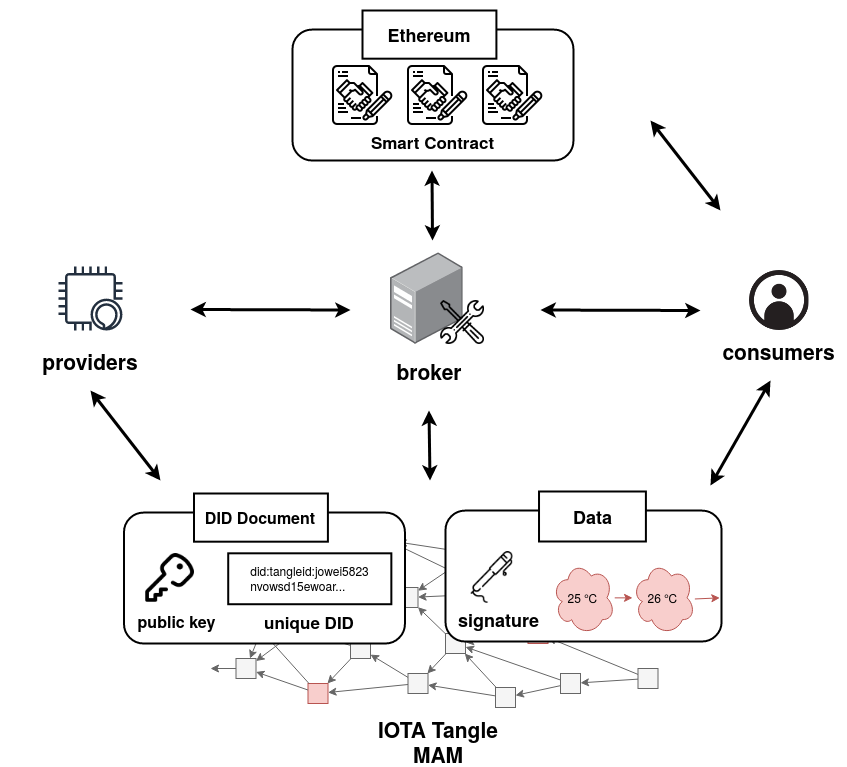
\includegraphics[width=3.in]{system_design}
    \caption{The system design of a decentralized data trading infrastructure which consists of data providers, consumers and brokers.}
    \label{fig:system_design}
\end{figure}

%TODO: cite IOTAIndustryMarketplace
\section{Related Work}
\label{section:relatedWork}
G. S. Ramachandran et al.\cite{trinity} pointed out the security risk of centralized brokers, and applied DLTs to build a distributed pub/sub system which promotes the transparency of interactions of participants and the status of data. The data validation and traceability are achieved via Ethereum smart contract. But data is plaintext on blockchain that the system is not appropriate for sensitive data.

Secure Pub-Sub model\cite{SPS}, a brokerless of pub/sub model, is proposed to eliminate the security risk of middleware and to provide a reputation-based fairness payment strategy on blockchain.
The privacy and data security are considered thoroughly with the encryption scheme, while the reputation of publishers, payment and data sharing are deployed on smart contracts that allows all operations are transparent. Yet, without brokers, participants may need to reveal more sensitive information in order to communicate. By Paolo Missier et. al\cite{MindMyValue} presenting an IoT brokered infrastructure based marketplace which enables trading with Ethereum smart contracts. The brokers are only responsible for data transmission in order to adapt flexible agreement between participants. However, the data cubes (i.e., a tuple of data information) are stored in a centralized Cassandra NoSQL database, which is guaranteed to be tamper-proof but the risk of single point failure still exists.

In the following researches, Masked Authenticated Messaging (MAM)\cite{MAM} is regarded as a secure data transmission layer and data storage built on top of DLT which provides access control, tamper-proof and authentication functionalities by tailoring messages to a channel. Jinzhi Lu et al.\cite{luDecentralizedDM} builds the data exchange system with MAM and IPFS\cite{IPFS}, a content-based addressing distributed storage system. With encrypted data contents storing on IPFS, and add the encrypted IPFS link to MAM for further exchange. A similar infrastructure proposed by Zichichi et al.\cite{SocialGood} offered a key and entry points management with MAM that minimize the information which data producers need to hold, and enable trading and perform access control on Ethereum smart contract. However, the details of trading and interactions between providers and consumers are not illustrated in this paper.

The industrial data marketplace\cite{IOTAIdustryMarketplace} proposed by IOTA Foundation targets for IoT data streams trading in IOTA token, and applies MAM as the data storage and data transmission layer. The decentralized data marketplace in \cite{DDMSmartCities} is fully decentralized without any intermediate server but data providers only, data providers attach and trade data streams via MAM. Nevertheless, the works above does not does not take into account the refund and unsubscribe mechanism of trading model.

 
\section{System Design Thinking}
\label{section:design_thinking}
\subsection{Data subscription-based trading platform players}
There are three major roles, data providers, data consumers and brokers which are similar to the pub/sub messaging model. But unlike the standard pub/sub model where brokers link the publishers and subscribers who are not aware of each others, in our proposed architecture, the brokers are only responsible for message delivery and essential verification processes.

\begin{itemize}
\item \textbf{Data Provider: }
Data providers are the ones that generate streaming data and set the data price based on the different types of data. With the subscription fee that earned via trading, data providers are incentivized to maintain and improve the quality of data.
\item \textbf{Data Consumer: }
Data consumers are entities that are willing to buy data streams. As it is laborious to widely deploy devices to collect data from scratch, and without a marketplace, it is also difficult to find providers of the data sets, purchases is the fastest and efficient way to get the desired data sets.
\item \textbf{Broker: }
Brokers are responsible for building an agreement between data providers and consumers. Also brokers can represent data providers to perform computing tasks as brokers are expected to have higher resource.
\end{itemize}

We adopt the brokered infrastructure for three reasons. Firstly, it inherits the benefits from the standard pub/sub model which is more efficient than the request/response model specifically in a large scale system. Furthermore, if either side is offline, the proceeding tasks have to stop and start over. With brokers, the unfinished work can be cached or accomplished. Second, a fully decentralized architecture has difficulties to brings data providers and consumers together, both of them need to reveal more sensitive information, such as IP address, in order to build the communication tunnel. The existence of brokers resolved the privacy issue, as brokers are the bridges that link data providers and consumers, participants can trade with minimum information like its identifier and public key. Third, as brokers running on machines in a stable network and electricity environment, participants on resource-constrained devices can offload the computation tasks to brokers that enables a proxy server implementation mentioned in Section~\ref{section:ta_endpoint}. With the end-to-end encryption trasmission protocol we used, brokers can perform verifiable checks without knowing the contents.

\begin{figure}[h]
    \centering
    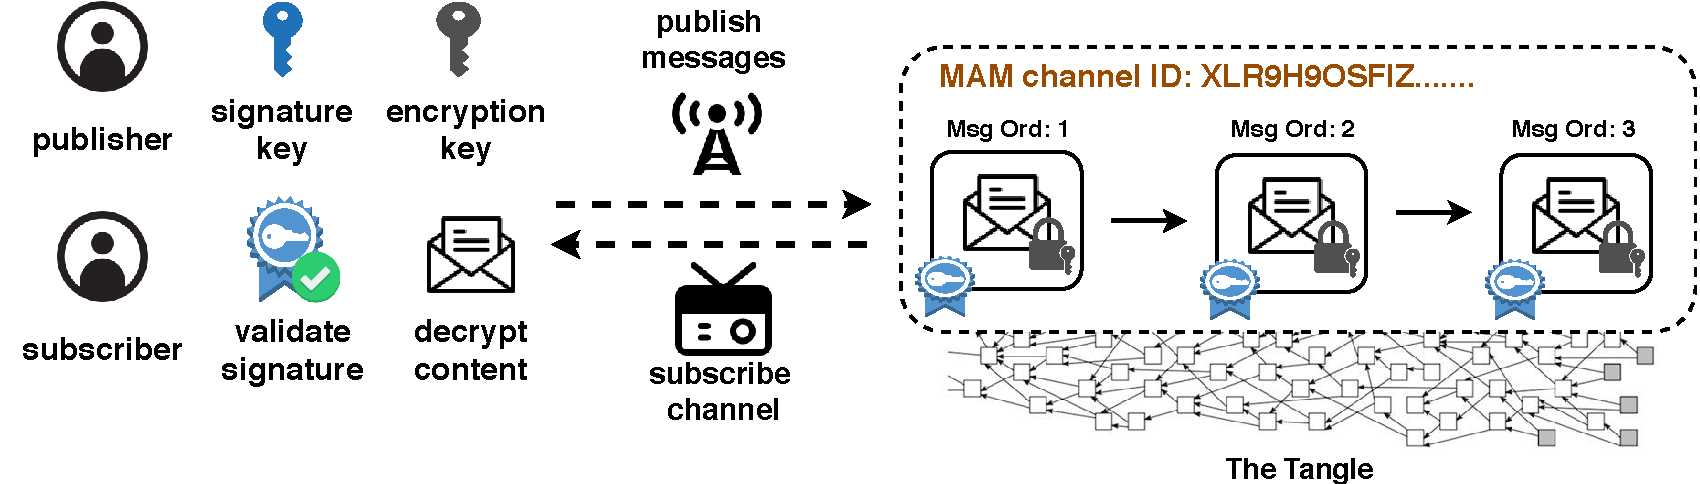
\includegraphics[width=3.5in]{channel_and_key_fold}
    \caption{Within MAM channel, the message publisher has 2 types of key, the encryption keys for content encryption and signature keys for digital signatures. Subscribers can validate the message with signature keys and decrypt messages with encryption keys.}
    \label{fig:channel_and_key}
\end{figure}


\subsection{Choice of Data Storage}
Data storage is the trust basis of data trading platforms where the data assets are reserved. Streaming data unlike a fixed set of data which can be verified by the hash of whole pack of data, it consists of continually granular records of each time slots. Therefore, the verification such as, data integrity and source identity are narrow down to a data point as well. In our proposed architecture, we adopt MAM as data storage to resolve the challenges of managing and verifying data streams. MAM is the second layer data communication protocol built on top of IOTA\cite{IOTAwhitepaper} network, the Tangle, a feeless cryptocurrency designed for IoT, which introduces properties like publishing, classifying and tracking authenticated message streams. Carrying these properties, MAM is also appropriate for building a self-sovereign identity system where the identity information such as public key, unique identifiers of services and metadata are stored. One can easily prove himself by sharing the identifier on MAM without any authority.

In our work, MAM build the trust of the platform while meeting the requirements of data trading which can be concluded below:

\begin{itemize}
    \item \textbf{Scalability}:
	\begin{itemize}
		\item Benefits from the underlying Tangle network, the system scales when more participants and more transactions join the network. 
    	\item For both data providers and consumers, MAM keeps the number of managed keys and data entry points as small as possible
    \end{itemize}    
    \item \textbf{Integrity}: 
	\begin{itemize}    	
        \item Messages published to the Tangle are tamper-proof that against malicious modification.
    	\item Messages are signed with the keys pre-generated under Merkle signature scheme\cite{MSS} (MSS) that both keys and messages can be verified by participants.
    \end{itemize}
    \item \textbf{Confidentiality}:
    \begin{itemize}    	
    	\item The encrypted data are uploaded that only participants that have keys can decrypt.
    	\item The authorized users can retrieve data streams, since data is written on the Tangle which can be queried as long as the IOTA network is alive.
    	\item MAM provides forward-secrecy. The entry points of future data can be derived, but it's impossible to trace back those in the past. This feature prevents adversaries from retrieving published history even if the key is revealed.
    \end{itemize}
\end{itemize}

MAM publishes authenticated streaming data to channel and endpoint as zero-value transactions to the Tangle and provides the ability to publish and fetch encrypted messages over the network along with data integrity and access control. The payload of a MAM message can be encrypted with an \textbf{encryption key} that restricts only authorized players can access contents, the ciphertext is then signed with \textbf{signature key} generated with MSS and attached to the Tangle. This approach allows users to validate the signatures without knowing the actual contents but ensuring the messages do come from the exact source. See Fig.~\ref{fig:channel_and_key} for illustration. 

Using MAM as a data storage benefits from the scalability of the underlying IOTA network as well as the decentralized and fault-tolerant characteristics of distributed ledgers, which reduce the risks of centralized storage services. Furthermore, the rights of data access are traded instead of a copy of data in the trading platform, which eliminates the need for data consumers to have additional storage.

\subsection{Digital Identity}
The digital identity represents an entity and holds the digital assets within the digital world, it is important to prove and show the identity to others during interactions. We select the decentralized identity model rather than a centralized one for the concerns in Table.\ref{tab:did}.

\begin{table}[h]
	\caption{The comparison of centralized and decentralized identity model}
	\label{tab:did}
	\begin{tabularx}{\linewidth}{|l|X|X|}
	\hline
		\textbf{Identity Model} & \textbf{Centralized} & \textbf{Decentralized} \\
		\hline
		Control & Enterprises control identities & Entities control their identities \\
		\hline
		Security & Identity held in a centralized service is a honeypot for cyber attacks & Decentralized identity limits data exposure \\
		\hline
		Portability & Identity is fragmented across enterprises & Identity can be portable across enterprises \\
		\hline
	\end{tabularx}
\end{table}

Centralized identity model may have single point failure in identifier management and security issues like data leakage. With sensitive information holding on certain authorities, whether the data leakage is caused by cyber attacks or unscrupulous organizations trading user data, the users' privacy are damaged. Furthermore, having a recognizable and portable identifier is important, otherwise, it is hard to cooperate fragmented identities of different data formats among institutions, and organizations may not approve identifiers of others.

In the decentralized identity model, every entity has a Decentralized Identifiers (DID\cite{DID} defined by W3C that contains identity information such as public key, unique identifiers of services and metadata. The digital footprints of entities is made up of Verifiable Credential (VC) added to their DIDs, issued by trusted issuers, such as schools and government departments. If a VC is verified via issuer's public key, the message will be labelled as trusted. Fig.~\ref{fig:did_vc} shows the relationship of VC issuer, verifier and user.

\begin{figure}[h]
    \centering
    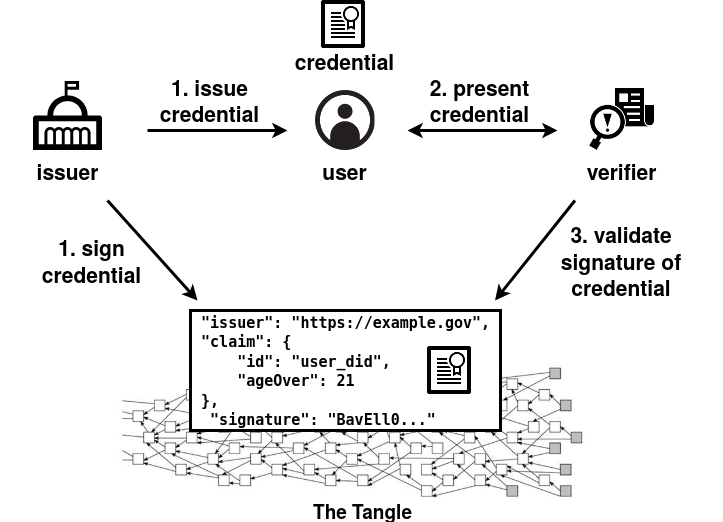
\includegraphics[width=3.in]{DID_VC}
    \caption{The trusted issuer requests user's DID, then issues a VC with his/hers signature. The user can then present the VC to verifier for signature validation.}
    \label{fig:did_vc}
\end{figure}

In our architecture, a decentralized identity system TangleID\cite{TangleID} is used, which is built on top of MAM where change logs of DIDs are traceable. One can easily prove himself by sharing the identifier on MAM without any authority.

Through TangleID, entities get a public/private key pair, the location of DID document and the seed (i.e., the identifier of its owner in IOTA) that generates the DID document MAM public channel. The public/private key pair can be used to exchange sensitive data and establish the trust communication, where messages that are encrypted with a public key can only be decrypted with private key owner. During data subscription process, the encryption keys of data products are encrypted with data consumers' public key on DID document which ensures only the subscribed consumers are accessible.

\subsection{Enable Automated Trading Process}
\begin{figure}[h]
    \centering
    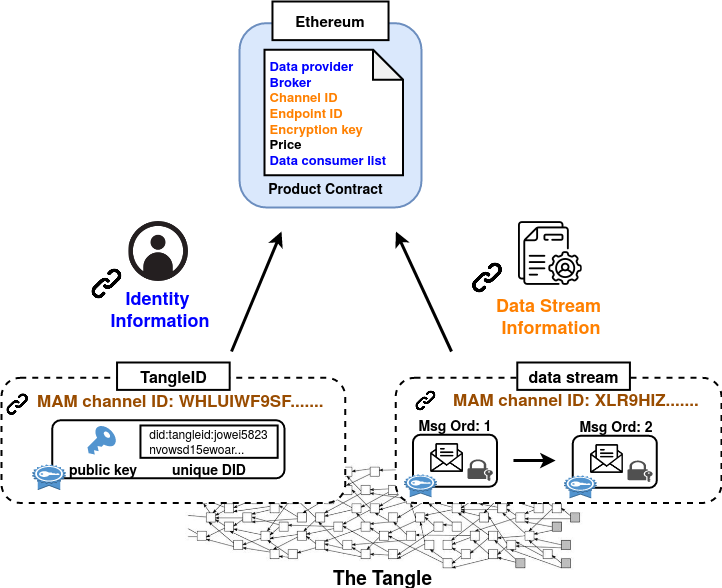
\includegraphics[width=3.5in]{smart_contract_mam_shrink}
    \caption{The information of identity and data streams are stored on the Tangle with MAM which are all recorded on Product Contracts. Participants can easily retrieve information via Product Contract and proceed trading. For signature validation check and further exchange encryption keys, the MAM channel ID of participants' DID document  are written down, presented in blue color. The orange color stands for the information of data products, which includes the data stream channel/endpoint ID and encryption key certified by broker.}
    \label{fig:smart_contract_mam}
\end{figure}

Ethereum is a cryptocurrency building on top of a public blockchain-based distributed ledger. It provides the smart contract, which is a protocol for formulating agreement on a blockchain that running on decentralized virtual machines. A smart contract can interact with other contracts, make decisions, store data and transfer cryptocurrency. All the participants in Ethereum can verify and execute the contracts, and once the contract is triggered, it is uninterruptible and will be executed automatically without any third-parties. 

With the functionalities of Ethereum smart contracts, a flexible and verifiable trading mechanism can be achieved. In our system, \textbf{Product Contract} is made for the product launching and trading. The information of data products such as address of the data provider, subscription fee, brokerage fee, threshold of consent votes of refunding, MAM channel/endpoint ID (the data entry point), time period and the broker-verified encryption key are listed on Product Contract. Fig.~\ref{fig:smart_contract_mam} shows the relationship of Product Contract and MAM. Furthermore, the participants can exchange encryption keys without any authorities via smart contracts. Though this design may cost extra transaction fees than exchanging key off-chain, it is considered a more secure strategy to protect the privacy of participants.

The transparency of smart contracts bring advantages for data providers and consumers. One of the advantage is that the trading states and progress are visible and verifiable which profits providers and consumers respectively. For data providers, with every details opened, the consumer list functions like a reputation evaluation, the better the quality the more the consumers he/her has. The consumer list and the states of products are key reputation referenced for data consumers to decide whether to subscribe. 

\subsection{Enable computation tasks delegation to broker with privacy}
To manage data products and to benefit from trading, data providers have to interact with MAM and Ethereum smart contract while doing its original tasks. However, the resources of low-level devices are precious which should be used to focus on its jobs. Therefore, the operations of MAM and smart contracts are better to be delegated to brokers. 

The delegation should ensure the privacy of data providers, for instance, brokers are asked to attach messages to MAM without knowing the contents as well as record encryption keys to smart contracts. To record encryption key to smart contract, data provider computes the digest of sensitive contents with hash function, and sends the digest as well as the signature to brokers. Broker can first verify the signature from data provider with the public key on DID document. If it's valid, then the broker uploads the key, otherwise the process will be aborted. Note that the broker needs to sign the messages he/she receives, which has been proven to be key uploaded by a broker recorded on the Product Contract. The number of key uploading time is also restricted in order to avoid data provider uploading fake key frequently. If the data consumers find out the encryption key does not match the signature or can not decrypt data streams as expected, they can launch a vote refund to withdraw their funds. Fig.~\ref{fig:key_upload} demonstrates the key uploading process to Product Contract via a broker. 

\begin{figure}[h]
    \centering
    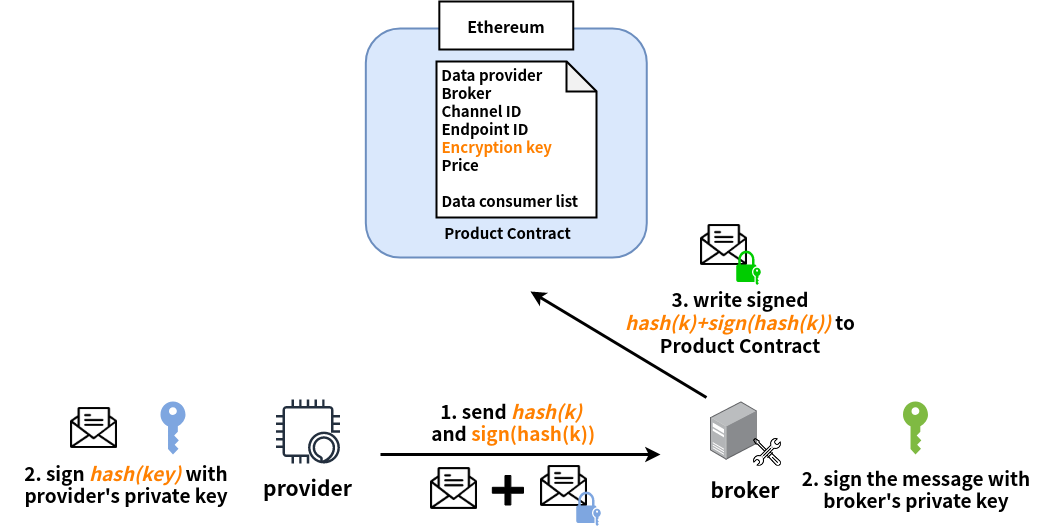
\includegraphics[width=3.5in]{key_upload}
    \caption{To add encryption key to Product Contract, the data provider sends the digest of encryption key and the one that signed with his/hers private key. After the broker receive the request, he/she performs digital signature as well, then write the result to the Product Contract.}
    \label{fig:key_upload}
\end{figure}

As for MAM operations, the performance results in Section.\ref{section:mam_performance} show that operating MAM costs a lot of resources for the devices, therefore, we present an alternative solution for data providers to delegate these computing tasks to powerful proxy servers, Tangle-accelerator\cite{TA}, while ensuring the privacy. The details would be further illustrated in Section.\ref{section:ta_endpoint}. 

\section{Masked Authenticated Messaging}
\label{section:MAM}
MAM enables broadcasting encrypted and authenticated data stream, referring as channel, on the Tangle. The publisher publishes messages that are propagated through the network and can be accessed by the subscribers only. With MAM, the rights of data access are traded instead of a copy of data in the trading platform, which eliminates the need for data consumers to have additional storage. 

\subsection{The Message Streams}
A channel/endpoint is a stream of MAM transaction bundles, which consist of signature and the masked message payload. To publish a MAM message to channel, MAM deploys MSS to sign the message payload to channel, where $channel\ ID = root$ i.e., the MSS Merkle root. The Merkle tree is generated with \textbf{seed}, an identifier of its owner in the IOTA protocol, represents the ownership of all things associated with the user in the IOTA ecosystem. Furthermore, the structure of channel/endpoint implements forward linking, each address of a message can be derived from the previous one that other entities can fetch the next payload. This design also brings the advantage of forward secrecy, where no one has access to the data back from his/her entry point. Figure.~\ref{fig:mam_structure} shows the structure of MAM channel/endpoint. 

\begin{figure}[h]
    \centering
    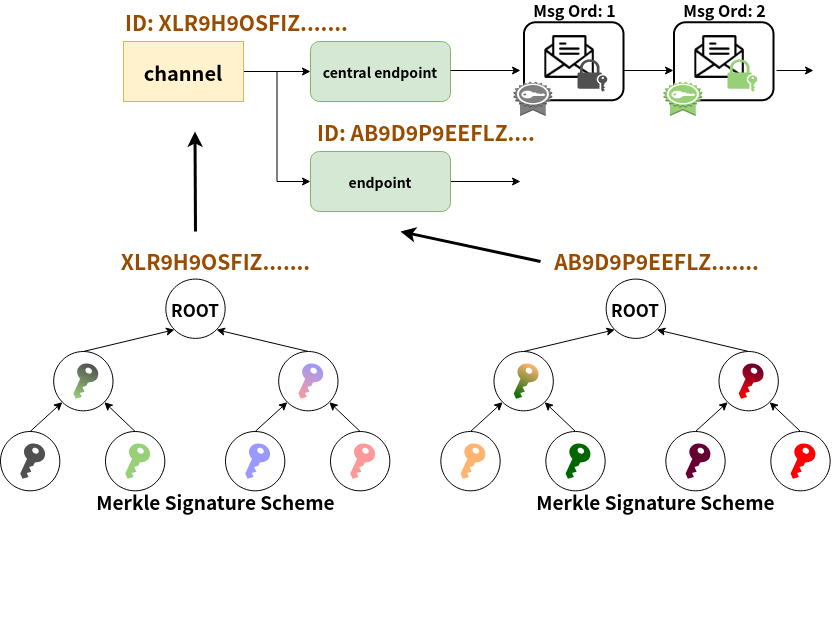
\includegraphics[width=3.5in]{mam_structure}
    \caption{With a seed, users can generate multiple channels, which can then generate multiple endpoints. The IDs of channel and endpoint are the roots of different Merkle trees in MSS. The "central endpoint" are endpoints that has ID, where $endpoint\ ID = channel\ ID$.}
    \label{fig:mam_structure}
\end{figure}

\subsection{Enable Access Control and Authentication}
The access control can be enabled via encryption with NTRU\cite{NTRU}, a quantum secure cryptosystem, or Pre-shared key (PSK), to prevent random users retrieving the data from channels. If the message payload is encrypted, subscribers are required for encryption keys to decode messages. The authentication in MAM includes two aspects: source and data. Source authentication ensures the message that originates from the claimed owner, and data authentication ensures the integrity of the data from the sender. These are achieved through the MSS and One-way hash functions by validating the signature added in the signature section of MAM bundle. However, the size of Merkle Hash Trees, that is, the size of a channel/endpoint should be determined at the start. Thus, data providers need to first decide how to distribute data products into MAM channels/endpoints before uploading data. 


\subsection{The Advantages of Adopting MAM in Subscription-based Data Trading Infrastructure}
%scalability
\subsubsection{A Scalable Keys and Data Entry Points Management}
The importance of scalable key and data entry points management increases over time. In MAM, with an entry point (i.e., the address of transaction) and the encryption key, one can derive the following addresses of transaction and retrieve data. Table.~\ref{tab:mam_scalability} compares the key and addresses that need to be managed by using MAM and other distributed storage systems. Assuming the length of data stream is 7, and each record is encrypted with the same key. With MAM, only 1 key and 1 entry point is required while other distributed storage need to reserve 7 entry points for each data record.

\begin{table}[htbp]
	\caption{Number of keys and entry points of a data stream that need to managed with length 7.}
	\label{tab:mam_scalability}
	\begin{center}
	\begin{tabular}{|c|c|c|}
	\hline
		\textbf{Items} & \textbf{MAM} & \textbf{Others} \\ 
		\hline
		keys & 1 & 1 \\ 
		\hline
		entry points & 1 & 7 \\ 
		\hline
	\end{tabular}
	\end{center}
\end{table}

%classify
\subsubsection{Data Sreams Classification}
The channel and endpoint structures enable users to be able to easily categorized data streams with respect to different types and usages. For instance, a voice assistant can create a channel every day with multiple endpoints for each gadgets to record daily logs. Another example is sensor devices like AirBox\cite{LASS}, collects environmental data, can split the statistics like PM 2.5 and humidity by time period into separate channels, which is useful for data providers to organize records and to pack into different data products. To do the classification in other distributed storage also encounters the aforementioned scalability problem.

%data trace
\subsubsection{A Traceable Data Stream}
Data traceability is an important security issue that allows users to track the changes of data. Currently, hash is widely used to generate checksums of entire package of files, users can compare the hash value of files in order to check the integrity. Yet the hash values of each new version are unrelated and it's hard to point out the differences between versions. MAM benefits from the singly linked-list data structure which attaches messages chronologically, users can easily track the footprints of data change logs as well as checking the validity of modifications with the signature.

\subsection{Delegate MAM operations to Tangle-accelerator}
\label{section:ta_endpoint}
MAM builds a secure and authenticated communication protocol on top of multiple cryptosystems, which low-level devices need to spend a lot of resources to apply it, and they may not even support built-in libraries in regular operating system. To overcome these concerns, we propose another approach that allows data providers to delegate the MAM operations to Tangle-accelerators, proxy servers with high computation power, which can accelerates the interactions with Tangle while ensuring the privacy of data providers. Fig.~\ref{fig:delegation} shows how data providers can adopt MAM.

\begin{figure}[!t]
    \centering
    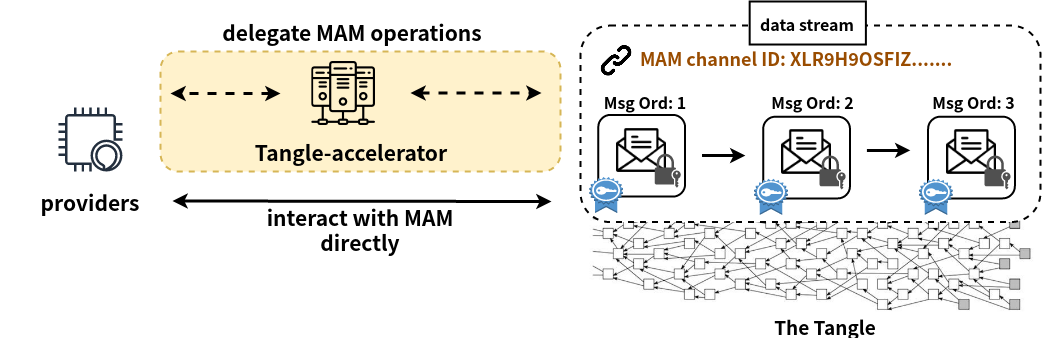
\includegraphics[width=\linewidth]{delegation}
    \caption{Data providers can use MAM in 2 ways: the provider performs MAM operations locally, and the provider delegates MAM operations to Tangle-accelerator.}
    \label{fig:delegation}
\end{figure}

\subsubsection{End-to-End-Encryption}
Introducing a proxy server to process all the cryptographic operations causes the proxy server or the middle man can easily tamper the message. To avoid such malicious operations during transmission, we introduce another lightweight end-to-end-encryption (E2EE) upon MAM protocol. The plaintext will be encrypted with this lightweight end-to-end-encryption. The E2EE process ensures only authorized subscribers can read the messages published on MAM.

%pic
\begin{figure}[!h]
    \centering
    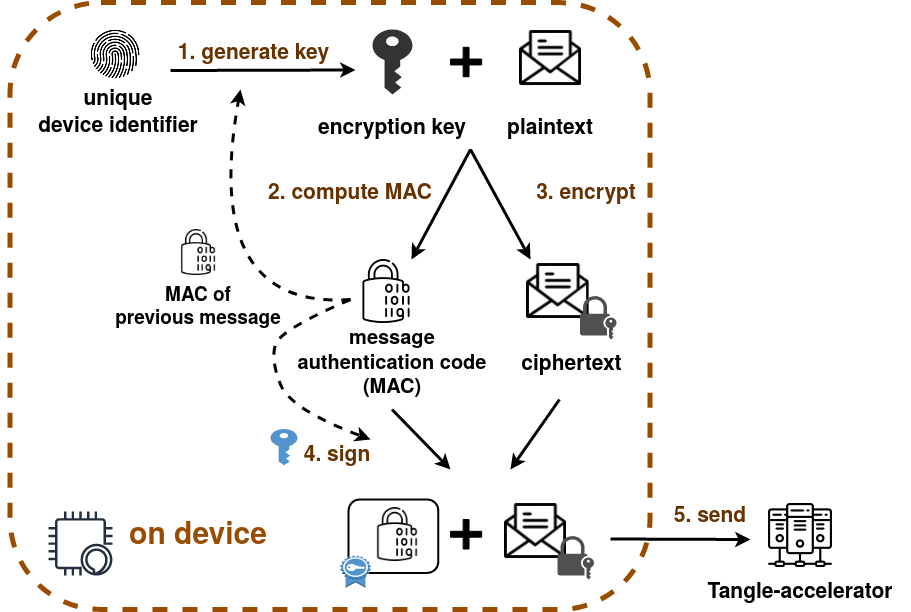
\includegraphics[width=3in]{MAM_E2EE_fold}
    \caption{The process of E2EE.}
    \label{fig:MAM_E2EE}
\end{figure}

In the Fig.~\ref{fig:MAM_E2EE}, we illustrate each step in the presented E2EE process. The details of steps are addressed below:

\begin{enumerate}
    \item Generate symmetric keys with unique device identifier and Message Authentication Code (MAC) of the previous message. If the message is the genesis message, then a sharing secret initialization information would serve as the MAC of previous message. Key Derivation Function (KDF) is used to generate the symmetric keys.
    \item Compute the Message Authentication Code (MAC) of current message with Hash-based Message Authentication Code(HMAC). Both plaintext and symmetric key would be given as parameters in HMAC.
    \item Apply the generated symmetric key to encrypt plaintext.
    \item Concatenate the MAC of current message would and the MAC of previous message, and then the result will be signed with digital signature algorithm.
    \item Send the ciphertext along with signed MAC.
\end{enumerate}

\begin{table}[htbp]
	\caption{AES256 Encryption Performance Numbers}
	\label{tab:AES_NI}
	\begin{center}
        \begin{tabular}{ |c||c|c|c|  }
            %\hline
            %\multicolumn{4}{|c|}{} \\
            \hline
            Size& \makecell{NON AES-NI \\ (msecs)} & \makecell{AES-NI \\ (msecs)} & \makecell{Encryption \\ Acceleration (\%)} \\
            \hline
            50 MB  & 1026  & 563   & 45.13 \\
            100 MB & 2036  & 1297  & 36.30 \\
            200 MB & 4282  & 2984  & 30.31 \\
            512 MB & 10754 & 6401  & 40.48 \\
            1 GB   & 23976 & 15721 & 34.43 \\
            \hline
        \end{tabular}
    \end{center}
\end{table}

The E2EE protocol presented in this paper combines a series of different cryptographic procedures. Each of them can be chosen on the basis of the working hardware and scenario by developers. On some certain devices, hardware acceleration would be supported. With hardware acceleration, the elapsed time could be dropped a step more. For example applying AES-NI can accelerate AES operations around 40\% on Intel devices.\cite{AES-NI-Acceleration} According to Intel, Table~\ref{tab:AES_NI} shows the performance of Encryption of AES256 with and without hardware acceleration.

\subsubsection{Issues in End-to-End-Encryption}
E2EE helps a lot for low-level edge device utilizing blockchain service. It dramatically reduces execution time encryption takes. However, there are some challenges in the E2EE process. Tampering the messages which have conducted E2EE would be a challenging mission. However, spamming would be the critical issue participants may meet under this architecture. It is risky for an edge device connects to a tangle-accelerator which is operated by unknown third-party. Sharing Channel Chain ownership with an unknown third-party would allow them to spam on the MAM Channel Chain. Spam would cause subscribers wasting plenty of time on decrypting useless messages. To prevent edge devices from the annoying attack, connecting to an known, trustworthy tangle-accelerator would be the easiest solution.

\section{Decentralized Subscription-based Data Trading Case Study}
\label{section:trading_model}
In this section, we illustrate how participants can join the data subscription platform, start subscribing, cancel subscription, and request refund.

\subsection{Prerequisite}
All participants are required to register on TangleID to get DID document and public/private key pair for sensitive contents exchange and authentication. An Ethereum account is also needed to interact with smart contracts and transfer Ethereum tokens.

\subsection{Launch Data Products}
To launch a data product, data providers need to create a MAM channel/endpoint for data streams and a Product Contract. For those resource-constraint IoT devices, the MAM related operations can be delegated to Tangle-accelerator, as mentioned in Section.~\ref{section:ta_endpoint}. And brokers are responsible for Product Contract creation. 

The details of data product, such as data price, MAM channel/endpoint ID and the length of data stream are listed on the Product Contract. As regard to the encryption key of data product, data providers send the hash digest of encryption key to a broker, who will then sign it and write it on the Product Contract. This provides an approach for data consumers to verify the encryption key that avoid data providers dishonest toward data consumers with a wrong one. The workflow is shown in Fig.~\ref{fig:launching_product}. Finally, the data product is launched and data providers can start uploading data.
 
\begin{figure}[!t]
    \centering
    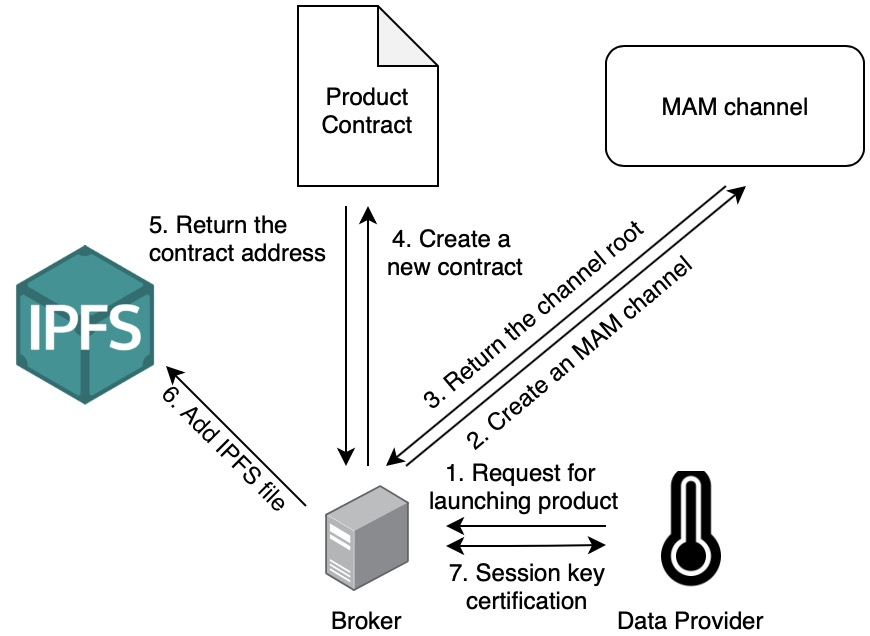
\includegraphics[width=2.5in]{launching_product}
    \caption{The process of launching a product.}
    \label{fig:launching_product}
\end{figure}

\subsection{Subscribe to Data Product}
Data consumers pay subscription fees to the Product Contract of desired data products, and data providers give the encryption key of data stream instead of the files to consumers. The MAM channel/endpoint encryption key is encrypted with the public key of data consumer by data provider and written on the Product Contract, which ensures only data consumers can decode it via Product Contract.

Transferring the encryption key on smart contract instead of off-chain not only ensures the consistency of the encryption key but also prevents frauds from malicious participants, and the exchange process is transparent to public. Furthermore, with the help of brokers and smart contracts, both data providers and consumers do not need to be online at the same time to proceed the trading process. The key sending process is shown in Fig.~\ref{fig:key_exchange}. The subscription fee is transferred from the Product Contract to data providers when the committed data is available on MAM.

\begin{figure}[!t]
    \centering
    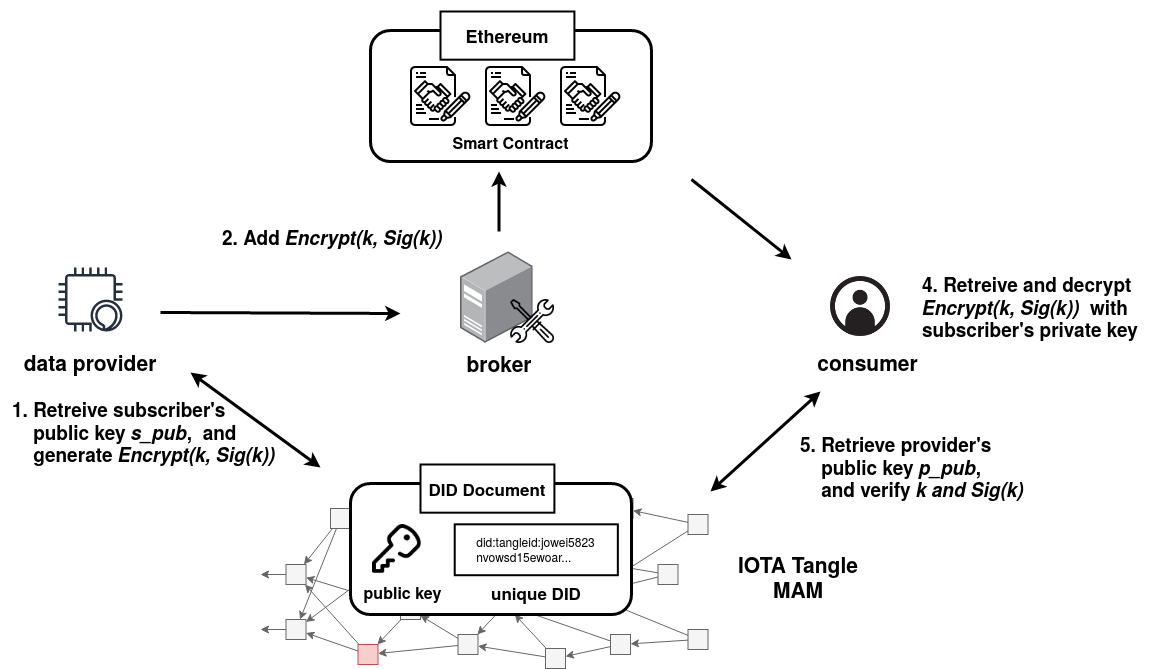
\includegraphics[width=3.5in]{key_exchange}
    \caption{Encryption key exchange process.}
    \label{fig:key_exchange}
\end{figure}

\subsection{Unsubscribe to Data Products}
Data consumers can unsubscribe to data products when they're not interested anymore. Product Contract marks the consumer as not subscribing, corresponding to the parameter $isSubscribe$ in $Product$ structre, since the delete function in Solidity does not remove the actual element but reseting it to default value. When data consumers trigger the unsubscribe event, a withdraw function is executed to pay subscription fee to providers and return the rest of the fee back to consumers. The amount of payment distributed to different players is defined in formula~\ref{equation:unsubscribe}. $i$ is the number of data when refunding condition is met, $price$  is the subscription price, $M$ is the number of expected data samples, $F_{b}$ (\%) is the brokerage fee which is expressed as a percentage, $F_{t}$ is the transaction fee of the smart contract, and $F_{cancel}$ is the cancellation fee charged for unsubscription. 

In SaaS, the cancellation fee is a way to make sure the service providers are protected. It is commonly used in pre-paid subscription-based services that allows service providers charge cancellation fee if subscribers drop out at the early stage. However, asking cancellation fee arbitrarily may cause an unfair contract that leads to the legal issue that should be carefully studied.

Also, data provider will change the encryption key of data product to prevent unsubscribers access to rest of the data. The new key should be updated to the remaining subscribers in $consumer2Purchase$ list in Product Contract.

\begin{gather}
\label{equation:unsubscribe}
    F_{DataProvider}(i) = price \frac{i-1}{M} (1-F_{b}+F_{cancel}) -F_{t} \\
    F_{Broker}(i) = price \frac{i-1}{M} F_{b} -F_{t} \\
    F_{Consumer}(i) = price (1-\frac{i-1}{M})(1 -F_{cancel}) -F_{t}
\end{gather}

\subsection{Launch a Refund}
Data subscription is a high risk which data provider may not upload data as the agreement set after receiving the subscription fee. Therefore, in our proposed architecture, data consumers can trigger a refund procedure by sending a transaction on Ethereum if the data is not available or defective. When the refund procedure is launched, all consumers vote to decide whether the refund is established. Once the ratio of consent votes of refunding is higher than a threshold, the subscription fee is proportionally transferred to the data provider, broker and every consumer as following.

\section{Evaluations}
\label{section:evaluation}
We evaluate the cost of operating the subscription-based data trading infrastructure in two aspects: 1) Evaluate the cost of adopting MAM on devices, since it is the most commonly used component to data provider. 2) Evaluate the minimum cost for participants to sustain or subscribe to a data product via Product Contract.

\subsection{MAM Performance Evaluation}
\label{section:mam_performance}
It is worth making a claim that all participants in data marketplace do not need to hold an IOTA full node which maintains the transaction history and exchanges information of the Tangle. Each role is only required to run client libraries and communicate with IOTA full nodes to interact with the Tangle. Therefore, in the following evaluations, all devices run with client library only.

MAM is a secure and validatable data storage of the proposed architecture. And publishing data to MAM is the primary key to resolve all the difficulties discussed in previous sections. The interactions between data providers and MAM can be frequent. Data providers can either upload data in a short time interval or maintain multiple MAM channels or endpoints at the same time, hence the operation of MAM is one of the potential bottleneck in data marketplace.

In this section, time measurement is evaluated in two MAM operations: channel/endpoint creation and data attachment to endpoints. To perform the evaluation assessment, a personal computer (PC, 3.2GHz 64-bit 6-core i7-8700 with 16GB DDR4 RAM) and a Raspberry Pi 3 Model B (1.2 GHz 64-bit quad-core ARM Cortex-A53 with 1GB LPDDR2 RAM) have been used to run MAM. 

\subsubsection{Channel / Endpoint Creation}
The length of a channel or endpoint is $2^{height}-1$ where \textit{height} is the height of Merkle Hash Tree in a Merkle signature scheme (MSS), and the "$-1$" is for announcing the ID of next channel or endpoint. A channel with height $n$ can create $2^n-1$ endpoints, and an endpoint with height $m$ can attach $2^m-1$ messages, therefore the capacity of a channel is $2^{nm}-2^n-2^m+1$ messages in total. The greater the \textit{height} of MSS, the longer the channel/endpoint, however the higher the computational power required. In this task, both channel and endpoint creation are tested and the \textit{height} is set from 1 to 7 which is quite enough for data providers to upload data.

Fig.~\ref{fig:mam_create} shows the results of channel/endpoint creation. The time duration for each \textit{height} is the average time of running 100 rounds. Since the creation of channel and endpoint are MSS calculations, the curves of the same hardware are nearly identical. On the other hand, the performance of Raspberry Pi 3 is acceptable when \textit{height} is smaller than 4, but time grows rapidly when \textit{height} is 5 or above. And the performance of PC remains acceptable even \textit{height} gets to 7. The results indicate that MAM channel/endpoint creation is a laborious job for a Raspberry Pi 3 when data providers need a longer channel/endpoint, which is one of the reason that MAM operations should be forwarded to brokers.
  
\begin{figure*}[!htb]
\minipage{0.32\textwidth}
  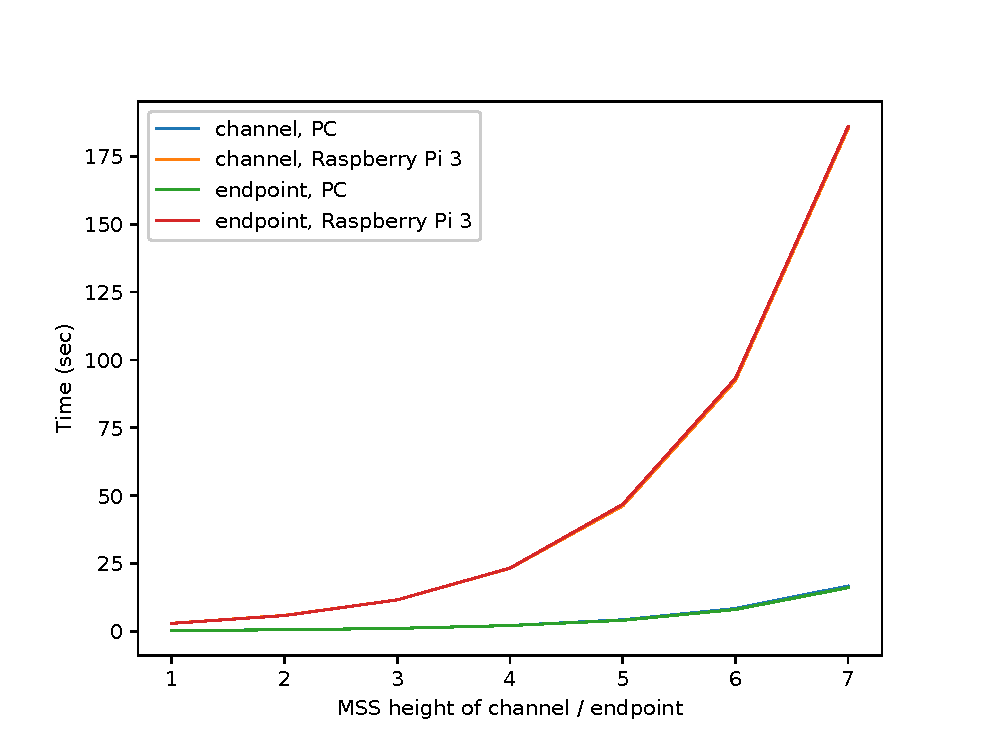
\includegraphics[width=\linewidth]{mam_create}
  \caption{Time cost of MAM creation.}\label{fig:mam_create}
\endminipage\hfill
\minipage{0.32\textwidth}
  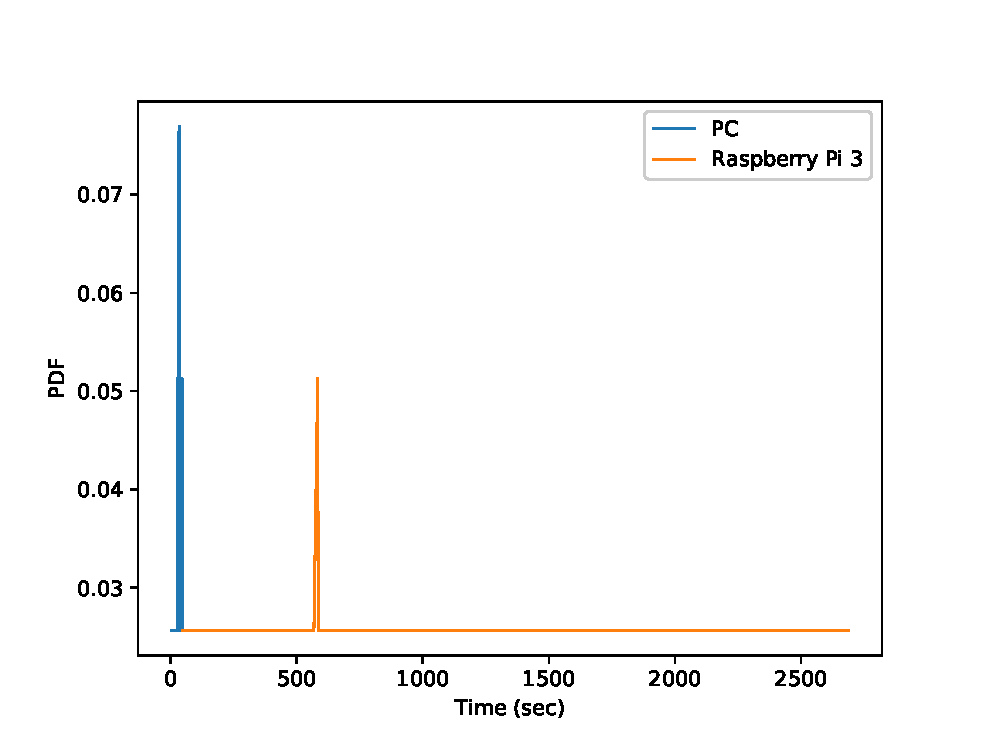
\includegraphics[width=\linewidth]{mam_send}
  \caption{The probability distributed function of time cost for sending a message through MAM.}\label{fig:mam_send}
\endminipage\hfill
\minipage{0.32\textwidth}%
  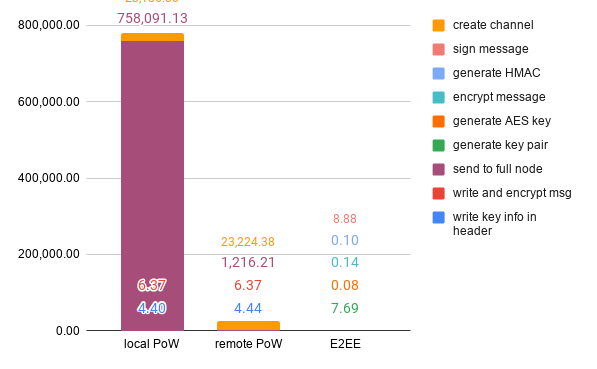
\includegraphics[width=\linewidth]{rpi3_pow}
  \caption{Local PoW vs. Remote PoW}\label{fig:rpi3_pow}
\endminipage
\end{figure*}

\subsubsection{Messages Publishment}
Publishing a message to MAM is attaching a zero-value transaction to the Tangle which requires two processes:
\begin{itemize}
	\item	Tips selection: In the IOTA protocol, a new-coming transaction needs to pick up 2 existed transactions called tips to reference and verify. The tips are provided by IOTA full nodes.
	\item	Proof-of-Work (PoW): An algorithm which prevents Denial of Service and spam attacks on a network. A computationally hard puzzle to solve, but easy to verify.
\end{itemize}

Tips selection requires a stable network connection to wait the response from IOTA full nodes, and PoW requires enough computation resources to perform. Fig.~\ref{fig:mam_send} shows probability distribution function of publishing a message to MAM endpoint. The time of Raspberry Pi 3 distributed widely, since the randomness of PoW has huge impact while all the tests on PC remain in a acceptable range.

The simulation results above indicate that MAM is difficult for low-level sensor devices to run, whereas these kind of devices are the majority hardware in the IoT scenarios. Furthermore, sensors with the low computing power and unstable internet connection are not able to have enough resources to handle data collection, data transmission on MAM and even trading process with subscribers simultaneously. 

Therefore, transferring MAM operations to brokers while ensuring the profit and privacy of providers through blind signatures can effectively solve performance problems and lower the threshold to participate in such framework. Brokers can be PCs or powerful machines that runs Ethereum client and Tangle-accelerator, where Ethereum client is used to interact with Ethereum and Tangle-accelerator provides PoW acceleration and MAM delegation. Fig.~\ref{fig:rpi3_pow} shows the time cost of sending a MAM message with local Pow on Raspberry Pi 3 and remote Pow on Tangle-accelerator. However, MAM operations still cost a considerable time that improving the performance of MAM is an essential issue that needs to be done for the next step.

\subsection{MAM vs. the delegated MAM}
\label{section:smart_contract_evaluation}

\subsubsection{Experiment}
Applying remote PoW greatly reduce the elapsed time. Channel creation is the next primary barrier for low-level devices to broadcast MAM message. With employing delegated MAM and E2EE, MAM channel creation would be delegated by tangle-accelerator which dramatically enhances the efficiency and makes MAM available for low-level devices. What follows is the performance comparison between MAM and delegated MAM (E2EE) for different payload sizes. Elapsed time for internet communication and PoW are not included, because the following processes starting from sending message to tangle-accelerator are the common steps. Excluding the common steps allows us to compare the performance between MAM and delegated MAM more clearly. In addition, MAM Channel creation and E2EE asymmetric key pair generation are not included, too. The two excluded steps take much more time than encrypting messages only, so counting these two steps would cause extreme values. In the E2EE protocol framework, we choose SHA-256 for HMAC, AES-CBC for symmetric encryption and Curve P-256 for ECDSA, respectively.

The steps counted in MAM benchmark including:
\begin{itemize}
	\item Encrypt input payload
	\item Publish final message on IOTA Tangle
\end{itemize}

The steps counted in E2EE benchmark including:
\begin{itemize}
	\item Generate symmetric key for encryption
	\item Hash input payload
	\item Encrypt input payload
	\item Transmit final message to tangle-accelerator
\end{itemize}

\begin{table}[htbp]
	\caption{Compare the performance between MAM and E2EE on Raspberry Pi}
    \label{tab:mam_vs_e2ee}
    \centering
        \begin{tabular}{|c||c|c|}
        \hline
            \textbf{size (bytes)} & \textbf{MAM(ms)} & \textbf{E2EE(ms)} \\
            \hline
            100 & 20.28 & 9.21 \\ 
            500 &  26.92 & 9.27 \\ 
            900 & 32.02 &  9.35  \\ 
            1300 & 36.67 & 9.41 \\ 
            1700 & 40.55 & 9.54 \\
            \hline
        \end{tabular}
\end{table}

It the Table~\ref{tab:mam_vs_e2ee}, a comparison of the two result reveals elapsing time of E2EE is obviously less than elapsing time of MAM which shows the E2EE process presented in the paper is a much more appropriate solution for resource-constrained systems to send authenticated streaming data.

\begin{gather}
    \label{eq:lin_mam_e2ee}
    y=0.0126 x+19.979 \\
    y=0.0002 x+9.174
\end{gather}

The equations in Eq.~\ref{eq:lin_mam_e2ee} are the linear equation for the experiment data of MAM and E2EE respectively. Apparently, the slope of the result of MAM is much greater than the result of E2EE. The small slope of E2EE ensures E2EE can consistently perform in an acceptable time range.

\subsubsection{Time Complexity}
With given E2EE protocol framework, ECDSA would take constant time under our situation, since the string needed to be signed is in fixed length. HMAC and AES-CBC are the procedures that cost most of the elapsed time. Time complexity of HMAC with SHA-256 is $O(n)$.\cite{hmac_time_complexity} Block cipher takes constant time for a single block which cause the time complexity is $O(n)$, too. Therefore, the E2EE protocol framework takes only linear time versus arbitrary string length. Applying mature cryptographic functions (e.g. SHA-256, AES-CBC, etc), ensures gentle slope as Eq.~\ref{eq:lin_e2ee} shows.

\section{Conclusion and Future Work}
\label{section:conclusion}
By combining the established standards and openly-developed specifications, this paper proposed an autonomous publish/subscribe model design to serve as a vendor and industry-neutral platform, automating the trading of digital assets and services. It was built with blockchain network, immutable audit trails, and contracts with an integrated decentralized identity system, to ensure the authenticity of all participants, enable secure communication and flexible trading mechanisms.

Some issues are worth discussing and improving. Brokers are the key to operate a stable system. However, we do not discuss the conditions that brokers are not responsive during trading process. It is worth studying the necessity of adoptin gossip protocol among brokers, which enables other brokers to continue the undone works. Search engine is needed to let consumers search and find interested data products, which might need an authority to design and run the service. 

\bibliographystyle{IEEEtran}
\bibliography{references}

\end{document}
